\documentclass{CML_Seminar_Template}

\begin{document}

\maketitle{Interruptions in HCI and Boundary Management}{\ }

\author{Andreas Rayzik}
       {Matrikelnummer 1891837}
       {andreas.rayzik@stud.uni-bamberg.de}

\begin{abstract}
Short abstract, max. 200 words  (Helvetica 10; height 13 Pt; 24 Pt above and below paragraph, centred). Abstract, abstract, abstract, abstract, abstract, abstract, abstract, abstract, abstract, abstract, abstract, abstract, abstract, abstract, abstract, abstract, abstract, abstract, abstract, abstract, abstract, abstract, abstract, abstract, abstract, abstract, abstract, abstract, abstract, abstract, abstract, abstract, abstract, abstract, abstract, abstract, abstract, abstract, abstract, abstract, abstract, abstract, abstract, abstract, abstract, abstract. 
\end{abstract}

\vspace{24pt}

\section{Introduction}

Job areas with on-call service mark a very interesting example of a boundary in which the consequences for unwanted transitions are especially high. The influences of constant interruptibility on mental and cognitive state become obvious. A questionnaire in 2006 and 2010 among Finnish physicians found that sleeping problems and WIF (work interference with family) lead to high distress, low job satisfaction and low work ability. The number of active on-call hours is associated with higher levels of WIF, but not with sleeping problems.
\par
Another study lists symptoms for mental, cognitive and behavioural effects. Table 1 shows a selection of symptoms. The kind of symptoms and their substantial prevalence among workers in on-call service shows the severity of the effects.

\subsection{Heading 2 (Times 14; 18 Pt above; 9 Pt below; flush left)}

Text in Times 12; height 15. No indenting for first paragraph. No indenting for first paragraph. No indenting for first paragraph. No indenting for first paragraph. 

\begin{itemize}
\item Bullet list (Times 12; height 15; indenting 5 mm) 
\item Bullet list (Times 12; height 15; indenting 5 mm) 
\end{itemize}

Subsequent paragraphs should have same font and layout, but with 5 mm indenting in the first line. 

\begin{enumerate}
\item Numbered list (Times 12; height 15; indenting 5 mm)
\item Numbered list (Times 12; height 15; indenting 5 mm)
\end{enumerate}
 
\subsubsection{Heading 3 (Times 12; 12 Pt above; 6 Pt below; flush left)}

Text in Times 12; height 15. No indenting for first paragraph. No indenting for first paragraph. No indenting for first paragraph. No indenting for first paragraph. 

And tables are referenced in the text like this (cf. Table ~\ref{CML_Seminar_Template_tab1}).

\begin{table}
\begin{center}
\begin{tabular}{ |c|c|} 
 \hline
 Key & Value \\
 \hline
 X & A \\
 \hline
\end{tabular}
\end{center}
    \caption{\label{CML_Seminar_Template_tab1} Table caption (Times 10; height 13 Pt; 12 above and below). Leave 12 Pt free above of the figure (use the same format for Tables, but with roman numbering). }
\end{table}

Subsequent paragraphs should have same font and layout, but with 5 mm indenting in the first line. 

\begin{quote}
Quotations with a length of more than 40 words should be put in a separate paragraph (Times 10; height 13; 2 Pt above; 2 Pt below; 5 mm indenting)
\end{quote}


Brands, company names, etc. should be written in capital letters (e.g., \textsc{The Coordinator}). The paper should have a length of about 16 pages. The pages should be numbered (page numbers in Helvetica 8; italic). Use a margin of 3.0 cm on the left and right side, and 2.5 cm on top and bottom. Refer to figures in the text (cf. Figure ~\ref{CML_Seminar_Template_fig1}).




References in the text should have the format [Author Year]. Sources with one author should be referenced as \cite[]{Gro1995}; sources with two authors like this \cite[]{MaVa1984}, and sources with more than two authors like this \cite[]{Ham2002}; if you have the page numbers, indicate them like this \cite[p. 16]{Gro1995} or this for a range \cite[pp. 16-17]{Gro1995}. 

\section{How paging technology enables high availability}
Pagers are small devices that are designed to be dedicated to the one task of delivering text messages quickly and reliably. Figure \ref{pager_fig1} shows an example of such a device. The interface elements on the front are very simple, with three arrow buttons for navigation and a power-on button. The display is a four-line alphanumeric monochrome display. The LCD has a back-light with adjustable contrast. It only displays the current date and time, and a message.
\par
Compared to a smartphone, the design is so much simpler and more efficient that the battery can be expected to last weeks instead of one or two days. The low-power CPU and the low-resolution monochrome display are the largest contributors to this feature. This is important in the case of a disaster, when there might be a power blackout and it is not possible to find a power outlet to charge a cellphone. The case of the device is sturdy and robust, so it can still function after being dropped from a moderate height. All of this contributes to a low-maintenance device, which on top of that can be quickly and inexpensively exchanged if it still gets lost or broken.

% TODO scale
\begin{figure}[htb]
  \begin{center}
   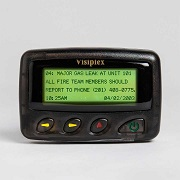
\includegraphics{pager_small.jpg}
  % \scalebox{.5}{\input{pager.jpg}}
  \end{center}
    \caption{\label{pager_fig1} An example of a paging device.}
\end{figure}

Paging technology operates in its own dedicated network. It has been proven to work during disasters, whereas the cellphone network tends to get overloaded and unreliable when many calls are being made. Paging provides encryption for data transport and over the air transmission. Compared to cellphone tower's signals, paging signals are more suitable to penetrate buildings. Additionally, they implement the so-called simulcast technology to combine signals for better reception.
\subsection*{Books:} 

\cite[]{Ham2002, MaVa1984}

\subsection*{Journals:}

\cite[]{Gro1995}

\subsection*{On-line Sources:} 

\cite[]{Bal1994}

\subsection*{Conference Proceedings:} 

\cite[]{GrPr2003}

\subsection*{Ph.D. and Master's theses:}

\cite[]{Dou1996}

\subsection*{Reports:} 

\cite[]{BeMa1993}


%\section*{Acknowledgements}
%
%\begin{acknowledgements}
%Acknowledgements. 
%\end{acknowledgements}

\bibliography{CML_Seminar_Template}

\end{document}
